%%Documentclass definition
\documentclass[xcolor=x11names,compress]{beamer} %beamer main class
%\documentclass[handout]{beamer} %for handouts

%%Package defintion
\usepackage{pgfpages}  %Printing multiple pages on one 
\usepackage{graphicx}  %Package 
\usepackage{tikz}      %Package for drawing
\usepackage{listings}
%\usepackage{hyperref}  %urls
\usepackage[utf8]{inputenc} 
\usepackage[ngerman]{babel}

%%
%% Beamer Layout %%%%%%%%%%%%%%%%%%%%%%%%%%%%%%%%%%
\useoutertheme[subsection=false,shadow]{miniframes}
\useinnertheme{default}
\setbeamertemplate{footline}{%
\begin{beamercolorbox}{section in head/foot}
    \color{gray}\vskip2pt~  \insertshorttitle\hfill\insertpagenumber{} %
    of \insertpresentationendpage{} ~\vskip2pt
\end{beamercolorbox}
}
\usefonttheme{serif}
\usepackage{palatino}

\setbeamerfont{title like}{shape=\scshape}
\setbeamerfont{frametitle}{shape=\scshape}

\setbeamercolor*{lower separation line head}{bg=DeepSkyBlue4} 
\setbeamercolor*{normal text}{fg=black,bg=white} 
\setbeamercolor*{alerted text}{fg=red} 
\setbeamercolor*{example text}{fg=black} 
\setbeamercolor*{structure}{fg=black} 
 
\setbeamercolor*{palette tertiary}{fg=black,bg=black!10} 
\setbeamercolor*{palette quaternary}{fg=black,bg=black!10} 

\setbeamertemplate{note page}[plain]

\renewcommand{\(}{\begin{columns}}
\renewcommand{\)}{\end{columns}}
\newcommand{\<}[1]{\begin{column}{#1}}
\renewcommand{\>}{\end{column}}
%%%%%%%%%%%%%%%%%%%%%%%%%%%%%%%%%%%%%%%%%%%%%%%%%%
%%

\title[Latex Beamer Einführung]{Einführung in Beamer\\Wie man eine Präsentation mit \LaTeX \,erstellt}
\author{Chi Trung Nguyen}
\institute{HfTL}
\date{5. März 2014}

\begin{document}

	\begin{frame}
		\titlepage
	\end{frame}

\frame{
	\frametitle{Inhaltsverzeichnis}
	\tableofcontents
	[pausesections]
}

\section{Warum \LaTeX\, Beamer?}
	\subsection{Vorteile}
		\begin{frame}{Vorteile}
			\begin{itemize}
				\item Wiederwendung von bereits erstellten Material
				\pause
				\item Versioncontrol
				\pause
				\item sehr gute und verständliche Dokumentation
			\end{itemize}

		\end{frame}

	\subsection{Nachteile}
		\begin{frame}{Nachteile}
			\begin{itemize}
				\item Zeitintensiv zu erlernen
				\pause
				\item Designs vorgegeben
				\pause
				\item Tabellen
				\pause
				\item Tabellen
			\end{itemize}
		\end{frame}

\section{Installation}
	\subsection{Itemize}
		\begin{frame}
			\begin{columns}
				\begin{column}[l]{5cm}
					\begin{block}{Windows}
						MikTex
					\end{block}
				\end{column}
				\pause
				\begin{column}[r]{5cm}
					\begin{block}{Mac}
						MacTex
					\end{block}
				\end{column}
			\end{columns}
		\end{frame}

\section{Basics}
	\subsection{Quellcode Beispiel}
	\begin{frame}[fragile]
	\frametitle{Quellcode Beispiel}
		\lstset{language=C++,
                keywordstyle=\color{blue},
                stringstyle=\color{red},
                commentstyle=\color{green},
                morecomment=[l][\color{magenta}]{\#}
		}
		\begin{lstlisting}
#include<stdio.h> 
#include<string.h>
string damn;

if (milkshake = my)
{
printf("bring all the boys to my yard");
damn="right";
}
		\end{lstlisting}
	\end{frame}	


	\subsection{Itemize}
		\begin{frame}{Auflistung}
			\begin{itemize}
				\item Item 1
				\pause
				\item Item 2
				\pause
					\begin{itemize}
						\item Verschachtelung
					\end{itemize}
			\end{itemize}
		\end{frame}

	\subsection{Bilder}
		\begin{frame}{Bilder}
			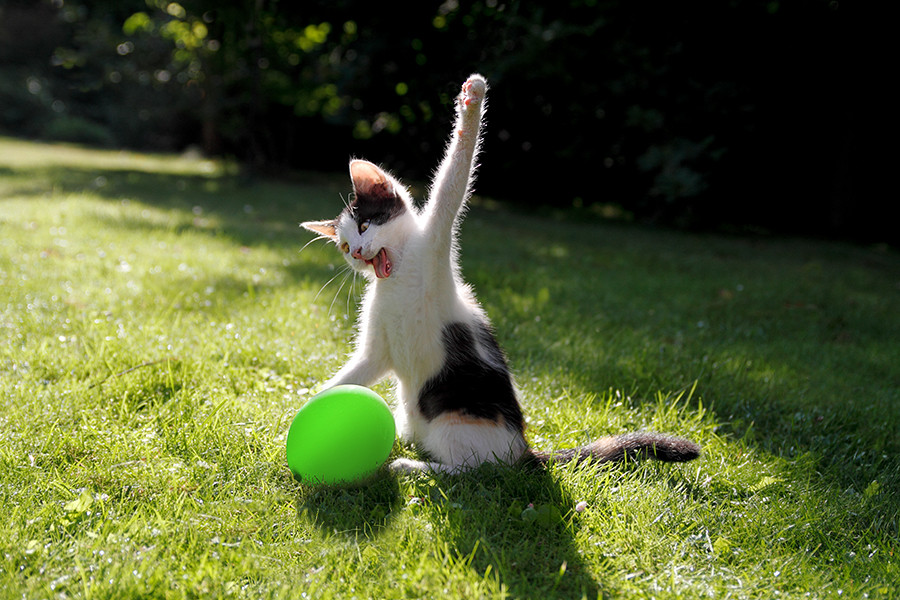
\includegraphics[width=300px]{images/IIctNxU.jpg}
		\end{frame}

	\subsection{Bilder}
		\begin{frame}{Bilder}
			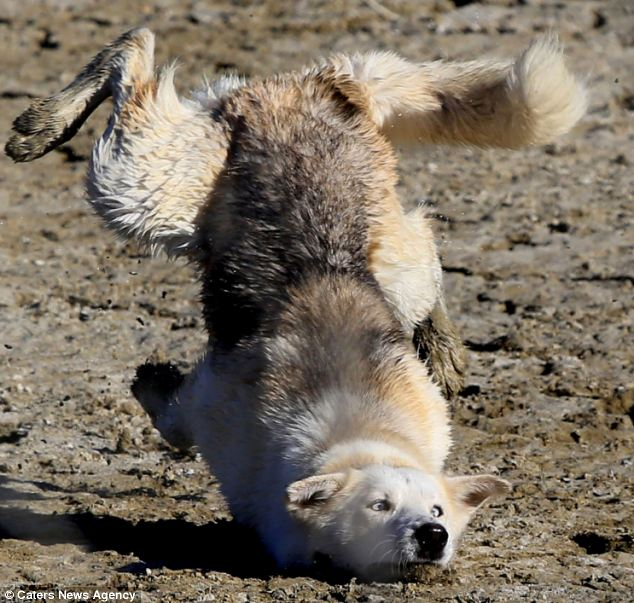
\includegraphics[width=200px]{images/GiSapDA.jpg}
		\end{frame}

	\subsection{Formel}
		\begin{frame}{mathematische Formeln}
			$$ \int_{-\infty}^\infty
e^{-x^2} \, dx = \sqrt{\pi}$$
		\end{frame}

	\subsection{Columns}
		\begin{frame}{Spalten}
			\begin{columns}
				\begin{column}[l]{5cm}
					\begin{block}{Spalte 1}
						\left(
						   \begin{array}{ccc}
						     a_{11} & \cdots & a_{1n} \\
						     \vdots & \ddots & \vdots \\
						     a_{m1} & \cdots & a_{mn}
						   \end{array}
						\right)
					\end{block}
				\end{column}
				\pause
				\begin{column}[r]{5cm}
					\begin{block}{Spalte 2}
						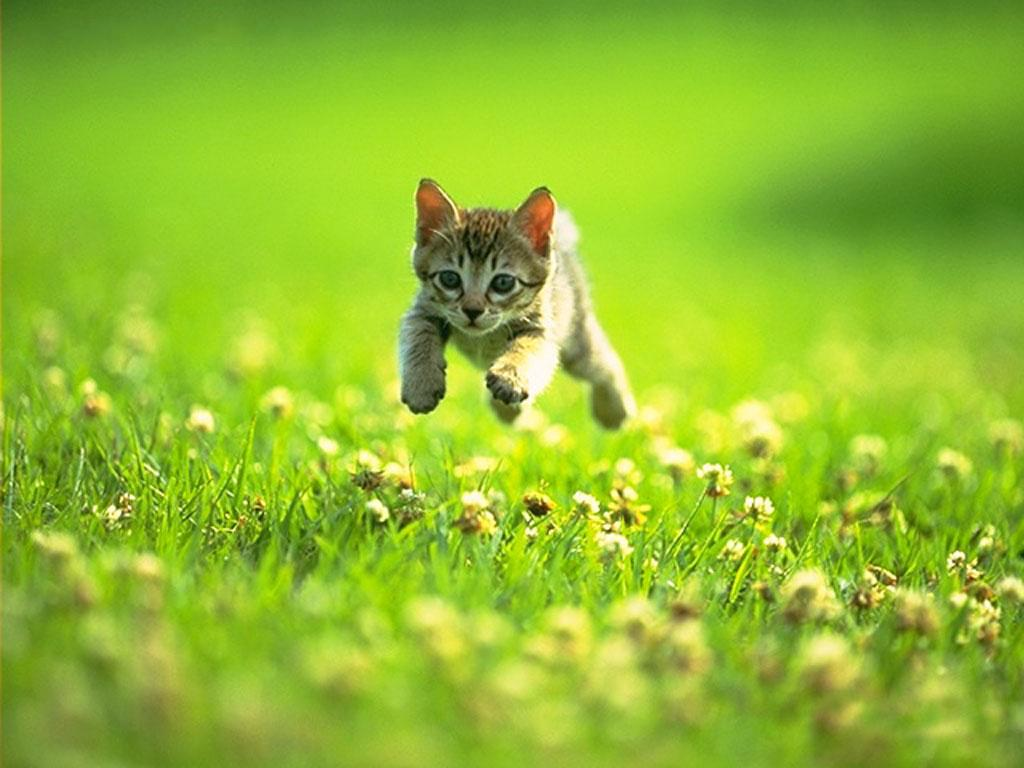
\includegraphics[width=0.5\textwidth]{images/cute-kitten-playing.jpg}
					\end{block}
				\end{column}
			\end{columns}
		\end{frame}

		\begin{frame}
			\begin{proof}
        Beweis
\end{proof}
		\end{frame}

\section{Fragen}
	\subsection{Quellcode}
		\begin{frame}
			Github Source und Präsentation:
			\href{http://s.ctnguyen.net/latex_hftl}{http://s.ctnguyen.net/latex\_hftl}
		\end{frame}

	\subsection{Fragen}
		\begin{frame}
			\huge{Fragen?}
		\end{frame}
\end{document}